$\{X(t):t \geq 0 \}$ is a continuous-time Markov chain since it satisfies the Markov property, i.e. 
$$P(X(t+s)=j|X(s)=i, X(u), 0 \leq u \leq s)=P(X(t+s)=j|X(s)=j)$$ 
for $i,j = 0,1,...$ and for all $s \geq 0$ and $t >0 $.

This is satisfied due to the fact that the sojourn times $S_S$, $S_L$ and $S_H$ is independent of each other and exponentially distributed, as given in the problem description.  OG NOE MED ONE STEP PROB

The jump probabilities are $P(S \rightarrow I_L)= 1 - \alpha$, $P(S \rightarrow I_H)= \alpha$, $P(I_L \rightarrow S)= P(I_H \rightarrow S) = 1$ and $P(I_L \rightarrow I_H)= P(I_H \rightarrow I_L) = 0$. 

The transition rates are found from formula $q_{ij} = P(i \rightarrow j ) q_i$, where $q_i = \sum_{j \neq i} q_{ij}$. Using $\alpha = 0.10$, this makes the transition probabilities $q_{SL} = 0.009$, $q_{SH} = 0.001$, $q_{LS} = 1/7$ and $q_{HS} = 1/20$. $q_{HL}=q_{LH}=0$ 

\begin{figure}
    \centering
    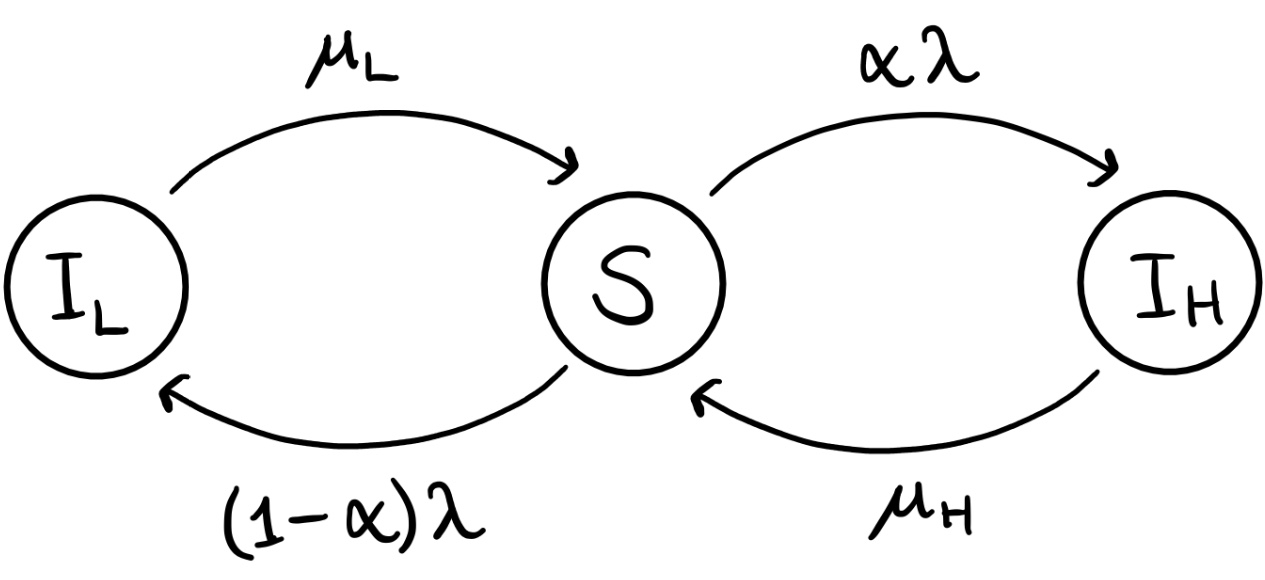
\includegraphics[width=90mm]{TransDiag1A.png}
    \caption{Transition diagram of $\{X(t):t\geq0\}$.}
    \label{plot_2a}
\end{figure}




